\subsection{Förderband Ballzuführung}
\begin{zebratabular}{p{4.5cm}p{\textwidth-3.6cm-0.7cm}}
    \rule{0pt}{11pt}\textit{Tester}           & Matteo Trachsel\\ 
    \rule{0pt}{11pt}\textit{Datum}:           & 26.03.2015   \\
    \rule{0pt}{11pt}\textit{Beschreibung}:    & Um die Bälle möglichst schnell zu den Beschleunigungsräder zu fördern, muss das Förderband gleichmässig, zentral und ohne Schlupf auf der Welle laufen. \\
    \rule{0pt}{11pt}\textit{Akteure}:         & Welle mit DC-Motor für Antrieb und Stirnrädern, Förderriemen mit aufgeklebten Leitschaufeln, Achse mit Spannelement. \\
    \rule{0pt}{11pt}\textit{Bedingung}:       & Funktionsmuster soweit montiert dass Förderreimen betrieben werden kann.\\
    \rule{0pt}{11pt}\textit{Erwartete Fehlermeldung}:          & keine \\
    \rule{0pt}{11pt}\textit{Vorgehen}:        & Förderreimen einsetzen, spannen, mit fünf Bällen bestücken. Spannung an DC-Motor anlegen. \\
    \rule{0pt}{11pt}\textit{Erwartetes Ergebnis}: & Bälle werden nach vorne befördert. Förderreimen bleibt mittig auf Achse und Welle (??***wort vergessen). Kein Schlupf zwischen Welle und Riemen. \\
    \rule{0pt}{11pt}\textit{Eingetretenes Ergebnis}: & Funktionsfähigkeit bestätigt. Erkenntnis: Schlupf auf Welle ist kein Problem. Je weniger der Riemen gespannt ist, desto gleichmässiger ist der Lauf. Keine Gefahr des seitlichen Ablaufens des Riemens. \newline
    Negativ: Durch ungenaue Bearbeitung läuft Stirnrad nicht Rund. 
    \\
    \rule{0pt}{11pt}\textit{Test bestanden?}:     & Ja, allerdings neues Stirnrad bestellen und nochmals bearbeiten.  \\
    \rule{0pt}{11pt}\textit{Weiter Tests nötig?}: & Nein \\
\end{zebratabular}  

\begin{figure}[h!]
	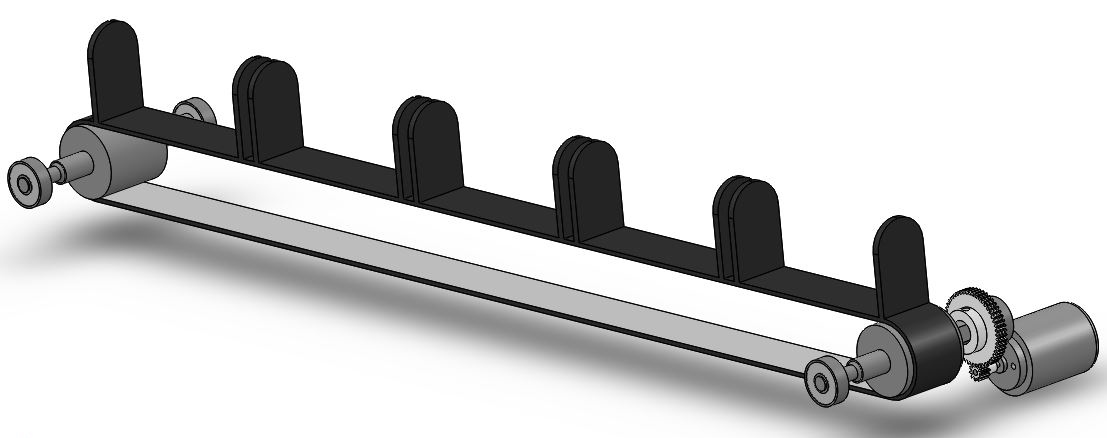
\includegraphics[width=0.5\textwidth,clip,trim=0cm 40cm 0cm 35cm]
	{Testberichte/Foerderband.jpg}
	\centering
	\caption{Förderband mit Führungschaufeln}
	\label{abb:Förderband mit Führungschaufeln}
\end{figure}